\begin{figure}[H]
\centering
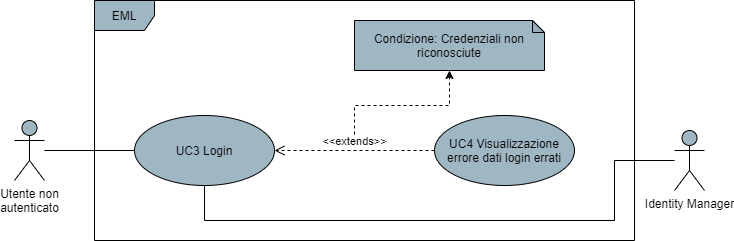
\includegraphics[scale=0.6]{res/UseCase/Immagini/Login}
\caption{Diagramma UML per modulo di login}
\end{figure}

\subsubsection{UCX - Login}
\begin{itemize}
\item \textbf{Attori primari}: utente non autenticato;
\item \textbf{Attori secondari}: identity manager;
\item \textbf{Descrizione}: l'utente, inserendo le proprie credenziali, viene autenticato alla piattaforma;
\item \textbf{Scenario Principale}: l'utente non ancora autenticato richiede l'accesso alla piattaforma dopo aver inserito le sue credenziali negli appositi campi dati. L'identity manager provvede alla validazione dei dati e l'utente viene autenticato.
\item \textbf{Specializzazioni}:
\begin{itemize}
	\item login cliente \textbf{[UCX.1]}
	\item login venditore \textbf{[UCX.2]}
\end{itemize}
\item \textbf{Estensioni}:
\begin{itemize}
	\item \textbf{UCX}: se le credenziali inserite non vengono riconosciute dall'identity manager, viene visualizzato un messaggio che informa l'utente dell'errore;
\end{itemize}
\item \textbf{Precondizione}: l'utente prova ad autenticarsi alla piattaforma;
\item \textbf{Postcondizione}: l'utente viene autenticato.
\end{itemize}

\subsubsection{UCX - Visualizzazione errore dati login errati}
\begin{itemize}
\item \textbf{Attori primari}: utente non autenticato;
\item \textbf{Attori secondari}: identity manager;
\item \textbf{Descrizione}: l'utente visualizza un messaggio di errore che lo informa che i dati da lui inseriti durante il login non sono riconosciuti dall'identity manager;
\item \textbf{Scenario Principale}: l'utente tenta di effettuare il login usando credenziali non presenti nel sistema;
\item \textbf{Precondizione}: l'utente prova ad autenticarsi alla piattaforma;
\item \textbf{Postcondizione}: viene visualizzato un messaggio che informa l'utente dell'errore di riconoscimento delle credenziali.
\end{itemize}

\subsubsection{UCX.1 - Login cliente}
\begin{itemize}
\item \textbf{Attori primari}: utente non autenticato;
\item \textbf{Attori secondari}: identity manager;
\item \textbf{Descrizione}: l'utente, inserendo le proprie credenziali, viene autenticato alla piattaforma come cliente;
\item \textbf{Scenario Principale}: l'utente non ancora autenticato richiede l'accesso alla piattaforma dopo aver inserito nel form apposito i dati richiesti \textbf{[UCX.1.1]}, premendo il pulsante di login \textbf{[UCX.1.2]}
\item \textbf{Precondizione}: l'utente prova ad autenticarsi alla piattaforma;
\item \textbf{Postcondizione}: l'utente viene autenticato come cliente.
\end{itemize}

\subsubsection{UCX.1.1 - Inserimento dati login cliente}
\begin{itemize}
\item \textbf{Attori primari}: utente non autenticato;
\item \textbf{Descrizione}: l'utente compila il form per il login;
\item \textbf{Scenario Principale}: l'utente inserisce i seguenti dati personali:
\begin{itemize}
	\item email \textbf{[UCX.1.1.1]};
	\item password \textbf{[UCX.1.1.2]}
\end{itemize}
\item \textbf{Precondizione}: il form di inserimento dati per il login è disponibile;
\item \textbf{Postcondizione}: i dati necessari al login sono stati compilati.
\end{itemize}

\subsubsection{UCX.1.1.1 - Inserimento email}
\begin{itemize}
\item \textbf{Attori primari}: utente non autenticato;
\item \textbf{Descrizione}: l'utente deve compilare il campo "Email" per procedere al login;
\item \textbf{Scenario Principale}: l'utente inserisce il suo indirizzo email nell'apposito campo;
\item \textbf{Precondizione}: il campo "Email" risulta vuoto;
\item \textbf{Postcondizione}: il campo "Email" è stato compilato.
\end{itemize}

\subsubsection{UCX.1.1.1 - Inserimento password}
\begin{itemize}
\item \textbf{Attori primari}: utente non autenticato;
\item \textbf{Descrizione}: l'utente deve compilare il campo "Password" per procedere al login;
\item \textbf{Scenario Principale}: l'utente inserisce la sua password nell'apposito campo;
\item \textbf{Precondizione}: il campo "Password" risulta vuoto;
\item \textbf{Postcondizione}: il campo "Password" è stato compilato.
\end{itemize}

\subsubsection{UCX.1.2 - Richiesta di login}
\begin{itemize}
\item \textbf{Attori primari}: utente non autenticato;
\item \textbf{Descrizione}: l'utente richiede l'autenticazione con i dati inseriti;
\item \textbf{Scenario Principale}: l'utente preme il tasto di login e manda la richiesta al sistema con i dati presenti nel form;
\item \textbf{Precondizione}: l'utente prova ad autenticarsi alla piattaforma;
\item \textbf{Postcondizione}: la richiesta di login è stata mandata al sistema;
\end{itemize}

\subsubsection{UCX.2 - Login venditore}
\begin{itemize}
\item \textbf{Attori primari}: utente non autenticato;
\item \textbf{Attori secondari}: identity manager;
\item \textbf{Descrizione}: l'utente, inserendo le proprie credenziali, viene autenticato alla piattaforma come venditore;
\item \textbf{Scenario Principale}: l'utente non ancora autenticato si trova nella pagina di login dedicata al venditore. Dopo aver inserito nel form apposito i dati richiesti \textbf{[UCX.2.1]}, preme il pulsante di login per autenticarsi \textbf{[UCX.2.2]}
\item \textbf{Precondizione}: l'utente prova ad autenticarsi alla piattaforma nella pagina dedicata al login per il venditore;
\item \textbf{Postcondizione}: l'utente viene autenticato come venditore.
\end{itemize}

\subsubsection{UCX.2.1 - Inserimento dati login venditore}
\begin{itemize}
\item \textbf{Attori primari}: utente non autenticato;
\item \textbf{Descrizione}: l'utente compila il form per il login;
\item \textbf{Scenario Principale}: l'utente inserisce nel form di login la password \textbf{[UCX.1.1.2]}
\item \textbf{Precondizione}: il form di inserimento dati per il login è disponibile;
\item \textbf{Postcondizione}: i dati necessari al login sono stati compilati.
\end{itemize}

\subsubsection{UCX.2.1.1 - Inserimento password}
\begin{itemize}
\item \textbf{Attori primari}: utente non autenticato;
\item \textbf{Descrizione}: l'utente deve compilare il campo "Password" per procedere al login;
\item \textbf{Scenario Principale}: l'utente inserisce la sua password nell'apposito campo;
\item \textbf{Precondizione}: il campo "Password" risulta vuoto;
\item \textbf{Postcondizione}: il campo "Password" è stato compilato.
\end{itemize}

\subsubsection{UCX.2.2 - Richiesta di login}
\begin{itemize}
\item \textbf{Attori primari}: utente non autenticato;
\item \textbf{Descrizione}: l'utente richiede l'autenticazione con i dati inseriti;
\item \textbf{Scenario Principale}: l'utente preme il tasto di login e manda la richiesta al sistema con i dati presenti nel form;
\item \textbf{Precondizione}: l'utente prova ad autenticarsi alla piattaforma nella pagina dedicata al login per il venditore;
\item \textbf{Postcondizione}: la richiesta di login è stata mandata al sistema;
\end{itemize}

